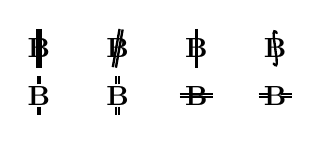
\begin{tikzpicture}
	\node[inner sep=0pt] at (0,0) {\textbf{B}};
	\draw[line width=0.3mm] (-0.02,7pt) -- (-0.02,-7pt);
	\draw[line width=0.3mm] (0.02,7pt) -- (0.02,-7pt);
	\node[inner sep=0pt] at (1,0) {\textbf{B}};
	\begin{scope}[xshift=1cm, rotate=-10]
	\draw[line width=0.3mm] (-0.02,7pt) -- (-0.02,-7pt);
	\draw[line width=0.3mm] (0.02,7pt) -- (0.02,-7pt);
	\end{scope}
	\node[inner sep=0pt] at (2,0) {\textbf{B}};
	\begin{scope}[xshift=2cm]
	\draw[line width=0.3mm] (0,7pt) -- (0,-7pt);
	\end{scope}
	\node[inner sep=0pt] at (3,0) {\textbf{B}};
	\begin{scope}[yshift=0cm, xshift=3cm]
	\draw[line width=0.3mm,line cap=round] plot [smooth, tension=1] coordinates { (0.02,5.5pt) (-0.02,5.5pt) (0,0) (0.02,-5.5pt) (-0.02,-5.5pt)};
	\end{scope}
	\node[inner sep=0pt] at (0,-0.6) {\textbf{B}};
	\begin{scope}[yshift=-0.6cm, xshift=0cm]
	\draw[line width=0.5mm] (0,4pt) -- (0,7pt);
	\draw[line width=0.5mm] (0,-4pt) -- (0,-7pt);
	\end{scope}
	\node[inner sep=0pt] at (1,-0.6) {\textbf{B}};
	\begin{scope}[yshift=-0.6cm, xshift=1cm]
	\draw[line width=0.3mm] (-0.02,4pt) -- (-0.02,7pt);
	\draw[line width=0.3mm] (0.02,4pt) -- (0.02,7pt);
	\draw[line width=0.3mm] (-0.02,-4pt) -- (-0.02,-7pt);
	\draw[line width=0.3mm] (0.02,-4pt) -- (0.02,-7pt);
	\end{scope}
	\node[inner sep=0pt] at (2,-0.6) {\textbf{B}};
	\begin{scope}[yshift=-0.6cm, xshift=2cm]
	\draw[line width=0.3mm] (-6pt,-0.02) -- (6pt,-0.02);
	\draw[line width=0.3mm] (-6pt,0.02) -- (6pt,0.02);
	\end{scope}
	\node[inner sep=0pt] at (3,-0.6) {\textbf{B}};
	\begin{scope}[yshift=-0.6cm, xshift=3cm]
	\draw[line width=0.3mm] (-6pt,-0.02) -- (-2.2pt,-0.02);
	\draw[line width=0.3mm] (-6pt,0.02) -- (-2.2pt,0.02);
	\draw[line width=0.3mm] (2.2pt,0.02) -- (6pt,0.02);
	\draw[line width=0.3mm] (2.2pt,-0.02) -- (6pt,-0.02);
	\end{scope}
\end{tikzpicture}
